\clearpage
\section{Gestione delle collection}
Le funzionalità di gestione delle \glossario{collection} elencate di seguito sono specificate nel \ManualeUtente{}:
	\begin{itemize}
		\item Visualizzazione \glossario{dashboard};
		\item Apertura \glossario{collection index};
		\item Apertura della \glossario{show page} di un \glossario{document};
		\item Visualizzazione \glossario{show page} attributi innestati.
	\end{itemize}
	

	\subsection{Modifica di un document da collection-index} %UCU 9.4
	\label{modificadocumentdacollectionindex}
		\begin{enumerate}

			\item Per modificare un \glossario{document} a partire dalla \glossario{collection-index} (Figura \ref{fig:modificadocumentdacollectionindex}) cliccare sul pulsante \emph{Edit} (1) relativo al documento che si vuole editare. 

				\begin{figure}[H]
					\centering 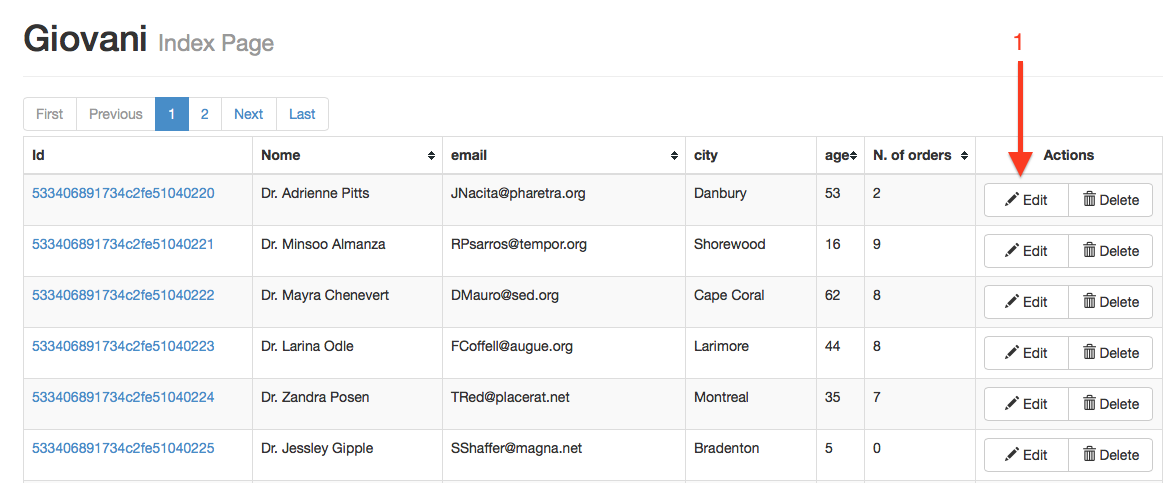
\includegraphics[width=1\textwidth]{img/modificadocumentdacollectionindex.png}
				\caption{\label{fig:modificadocumentdacollectionindex} Pulsante modifica collection da collection-index}
				\end{figure}

			\item \label{modificaDocumentForm} La pagina di modifica del \glossario{document} (Figura \ref{fig:modificaDocumentForm} permette l'edit degli attributi disponibili (1), (2). Per salvare le modifiche cliccare sul pulsante \emph{Save changes} (3). Se l'utente desidera interrompere l'operazione di modifica, perdendo così i dati non salvati, cliccare sul pulsante \emph{Cancel} (4). 

				\begin{figure}[H]
					\centering 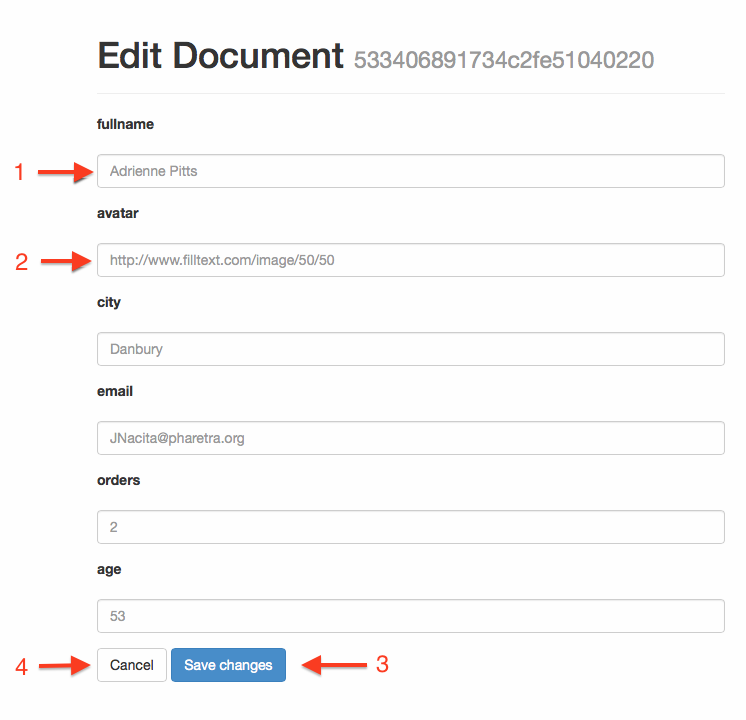
\includegraphics[width=0.8\textwidth]{img/modificaDocumentForm.png}
					\caption{\label{fig:modificaDocumentForm} Form di modifica document}
				\end{figure}

		\end{enumerate}

	\clearpage
	\subsection{Modifica di un document da show-page} %UCU 9.1.3
	\label{modificadocumentdashowpage}

			Per modificare un \glossario{document} a partire dalla relativa show-page (Figura \ref{fig:modificadocumentdashowpage}) cliccare il pulsante \emph{Edit Document} (1). Il sistema presenterà un form con il quale è possibile modificare gli attributi disponibili (vedi \ref{modificaDocumentForm}).

				\begin{figure}[H]
					\centering 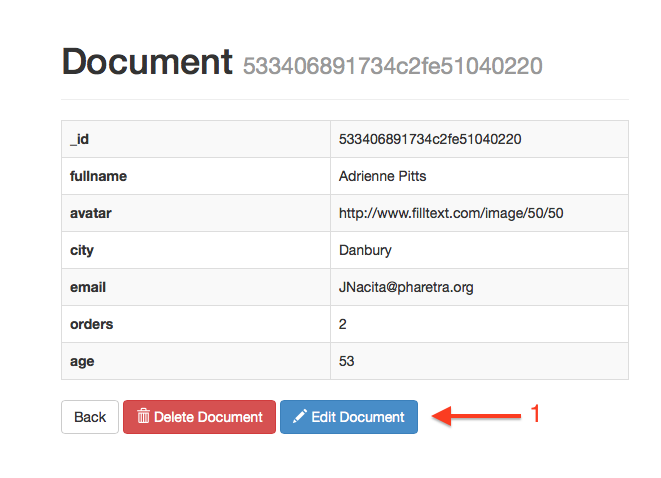
\includegraphics[width=0.8\textwidth]{img/modificadocumentdashowpage.png}
				\caption{\label{fig:modificadocumentdashowpage} Modifica di un document da show-page}
				\end{figure}
	
	\clearpage
	\subsection{Eliminazione di un document da collection-index} %UCU 9.5
	\label{eliminadocumentdacollectionindex}
		\begin{enumerate}
			\item Per eliminare un \glossario{document} a partire dalla \glossario{collection-index} (Figura \ref{fig:eliminadocumentdacollectionindex}) cliccare sul pulsante \emph{Delete} (1).

					\begin{figure}[H]
						\centering 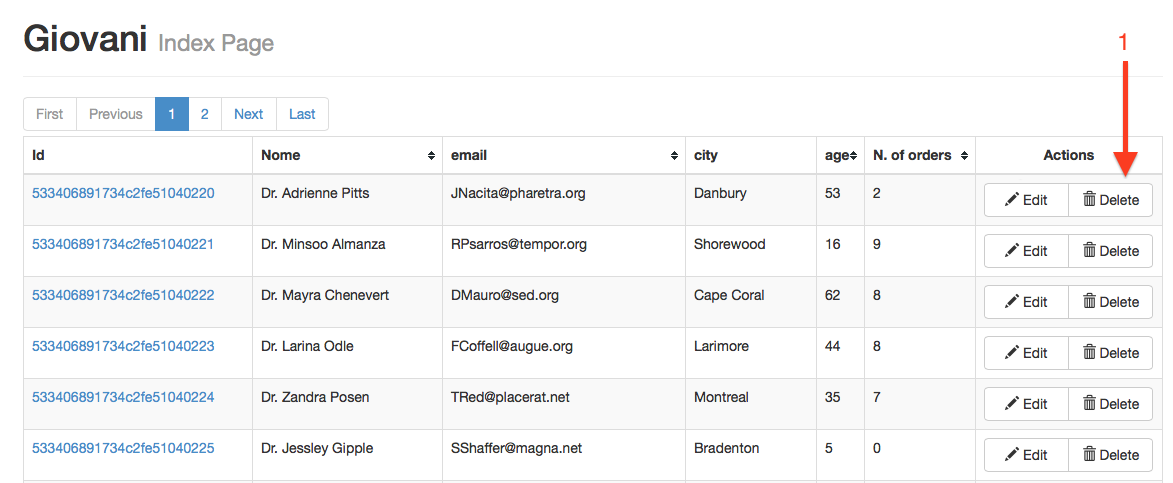
\includegraphics[width=0.8\textwidth]{img/eliminadocumentdacollectionindex.png}
					\caption{\label{fig:eliminadocumentdacollectionindex} Pulsante per eliminare un document da collection-index}
					\end{figure}

			\item \label{confermaEliminazDocument} Confermare l'eliminazione del \glossario{document} tramite la finestra proposta dal browser (Figura \ref{fig:confermaEliminazDocument}).
					\begin{figure}[H]
							\centering 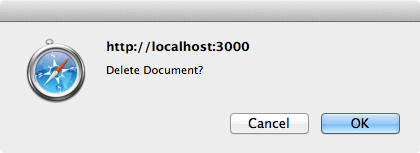
\includegraphics[width=0.6\textwidth]{img/confermaEliminazDocument.png}
					\caption{\label{fig:confermaEliminazDocument} Finestra conferma eliminazione document}
					\end{figure}

		\end{enumerate}
	
	\clearpage
	\subsection{Eliminazione di un document da show-page} %UCU 9.1.4
	\label{eliminazionedocumentdashowpage}

			Per eliminare un \glossario{document} a partire dalla relativa \glossario{show page} (Figura \ref{fig:eliminazionedocumentdashowpage}) cliccare il pulsante \emph{Delete Document} (1). Confermare l'eliminazione come indicato in \ref{confermaEliminazDocument}.

				\begin{figure}[H]
					\centering 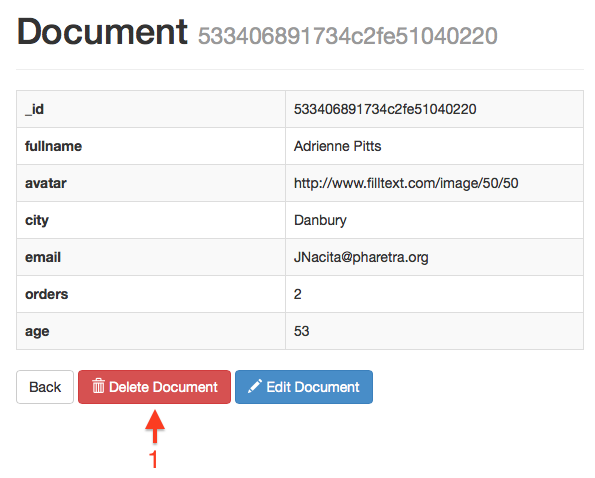
\includegraphics[width=0.8\textwidth]{img/eliminazionedocumentdashowpage.png}
				\caption{\label{fig:eliminazionedocumentdashowpage} Pulsante per eliminare un document da show-page}
				\end{figure}

